\documentclass[conference]{IEEEtran}
\usepackage{cite}
\usepackage{amsmath,amssymb,amsfonts}
\usepackage{algorithmic}
\usepackage{graphicx}
\usepackage{textcomp}
\usepackage{xcolor}
\usepackage{booktabs}
\usepackage{multirow}
\usepackage[hidelinks]{hyperref}
\usepackage{fancyhdr}

\def\BibTeX{{\rm B\kern-.05em{\sc i\kern-.025em b}\kern-.08em
    T\kern-.1667em\lower.7ex\hbox{E}\kern-.125emX}}

\pagestyle{fancy}
\fancyhf{}
\renewcommand{\headrulewidth}{0pt}
\fancyfoot[R]{\thepage}

\begin{document}

\title{Data Mining the Bavarian Card Game Schafkopf: Extracting Actionable Playing Rules Through Machine Learning}

\author{\IEEEauthorblockN{Anonymous Author}
\IEEEauthorblockA{\textit{Department of Computer Science} \\
\textit{University Name}\\
City, Country \\
email@example.com}}

\maketitle

\begin{abstract}
We present a comprehensive data mining study of Schafkopf, a traditional Bavarian trick-taking card game, extracting actionable playing rules from over 73,000 game states and 30,000 unique hand configurations. Using an ensemble of eight data mining algorithms—including decision trees, association rule mining, clustering, and gradient boosting—we discover statistically significant patterns that challenge conventional wisdom. Our key findings include: (1) trump count exhibits a strong correlation ($r = 0.794$) with win probability while total points show near-zero correlation ($r = 0.066$), contradicting the intuition that high-point hands are stronger; (2) a clear ``4-trump threshold'' rule where hands with four or more trumps achieve $>$55\% win rate; (3) early-game card plays have 37\% error rates compared to 4\% in late game, indicating that strategic decisions compound throughout gameplay. We validate discovered rules through Monte Carlo simulation on 43,420 decision points, achieving 87.3\% accuracy in predicting optimal bidding decisions. This work demonstrates the application of knowledge discovery techniques to traditional card games, providing both scientific insights and practical guidelines for players.
\end{abstract}

\begin{IEEEkeywords}
data mining, Schafkopf, card games, decision trees, association rules, knowledge discovery, rule extraction, machine learning, game analytics
\end{IEEEkeywords}

\section{Introduction}

Traditional card games represent a rich domain for data mining research, combining stochastic elements, hidden information, and complex strategic decisions. While games like Poker have received extensive attention from the research community \cite{billings2002challenge}, many culturally significant games remain understudied from a data science perspective. This work addresses this gap by applying comprehensive data mining techniques to Schafkopf, a traditional Bavarian trick-taking card game with over 200 years of history.

Schafkopf presents unique challenges for knowledge discovery. Unlike games with complete information such as Chess, players must reason under uncertainty about opponent holdings. The game features dynamic team formation where partnerships may remain hidden, creating complex strategic considerations. Traditional expert knowledge about Schafkopf has been passed down through generations, but systematic data-driven validation of these heuristics has been lacking.

The application of data mining to traditional card games offers several benefits. First, it can validate or refute conventional wisdom with statistical rigor. Second, it can discover non-obvious patterns that escape human intuition. Third, it preserves cultural knowledge in quantitative form that can be analyzed, taught, and transmitted reliably. Finally, insights from game analysis often generalize to other decision-making domains under uncertainty.

Our research addresses the following questions:
\begin{enumerate}
    \item What hand characteristics most strongly predict game outcomes?
    \item Can we extract interpretable, actionable rules for bidding decisions?
    \item What card play patterns lead to suboptimal decisions?
    \item Do machine learning algorithms validate or contradict traditional expert wisdom?
\end{enumerate}

We employ an ensemble of eight data mining algorithms to analyze two complementary datasets: 30,000 unique hand configurations with Monte Carlo-estimated win rates, and 43,420 in-game decision points with optimal action labels. Our key contributions include:

\begin{itemize}
    \item Discovery of the ``4-trump threshold''—a statistically validated bidding rule with 87.3\% predictive accuracy
    \item Quantitative evidence that trump count dominates point count (correlation ratio 12:1) in determining hand strength
    \item Identification of error-prone game phases and card play patterns through association rule mining
    \item A validated set of six actionable rules for human players derived from machine learning models
\end{itemize}

\section{Background}

\subsection{Schafkopf Rules and Terminology}

Schafkopf is played with four players using a 32-card German deck consisting of four suits (Acorn, Leaf, Heart, Bell) and eight ranks (7, 8, 9, 10, Unter, Ober, King, Ace). In the standard ``Sauspiel'' (partner game) mode, one player becomes the declarer by calling an Ace, and the holder of that Ace becomes the declarer's hidden partner.

The trump hierarchy in Schafkopf is distinctive. All Obers (Queens) and Unters (Jacks) are permanent trumps ranked: O-Acorn $>$ O-Leaf $>$ O-Heart $>$ O-Bell $>$ U-Acorn $>$ U-Leaf $>$ U-Heart $>$ U-Bell. Hearts additionally serve as the trump suit, giving 14 total trump cards. Point values are: Ace=11, 10=10, King=4, Ober=3, Unter=2, others=0, totaling 120 points. The declarer team wins by capturing at least 61 points.

\subsection{Related Work in Game Data Mining}

Data mining has been successfully applied to various games. In Poker, pattern mining has revealed betting behaviors and bluffing patterns \cite{billings2002challenge}. Chess databases have been analyzed to understand opening repertoires and strategic trends \cite{silver2016mastering}. For trick-taking games specifically, research on Bridge \cite{tian2020joint} and Skat \cite{kupferschmid2006skat} has employed machine learning for bidding and play decisions.

Association rule mining, originally developed for market basket analysis \cite{agrawal1994fast}, has found applications in game log analysis. Decision tree algorithms \cite{quinlan1986induction} are particularly valuable for game domains due to their interpretability. Clustering techniques have been used to categorize player strategies and game states in various domains.

\section{Methodology}

\subsection{Data Collection}

We collected two complementary datasets for analysis:

\textbf{Hand Strength Dataset}: 30,000 unique hand configurations, each evaluated through 100 Monte Carlo simulations. For each hand, we recorded:
\begin{itemize}
    \item Trump count (0-8 trumps possible)
    \item Strongest trump rank (1=O-Acorn, 14=no trumps)
    \item Total card points in hand
    \item Maximum suit run (consecutive cards in one suit)
    \item Empirical win rate from simulations
\end{itemize}

\textbf{Decision Point Dataset}: 43,420 in-game decision states from 2,000 complete games played by a rule-based agent. For each state, we recorded the current game context, the agent's chosen action, and Monte Carlo-evaluated optimal actions with Q-values.

\subsection{Data Mining Algorithms Applied}

We employed eight complementary algorithms, each selected for its unique analytical strengths and ability to reveal different aspects of game strategy:

\subsubsection{Decision Tree (CART)}
Classification and Regression Trees \cite{breiman1984classification} recursively partition the feature space using binary splits that maximize information gain. For Schafkopf bidding, CART identifies the most discriminative hand features and their threshold values. We configured the algorithm with maximum depth of 4 levels to maintain interpretability, minimum 100 samples per leaf to ensure statistical reliability, and Gini impurity as the splitting criterion. The resulting tree structure directly translates into human-readable if-then rules.

\subsubsection{Association Rule Mining (Apriori)}
The Apriori algorithm \cite{agrawal1994fast} discovers frequent itemsets and derives association rules of the form $X \Rightarrow Y$ with confidence and lift metrics. We discretized continuous features (e.g., trick number into ``early,'' ``middle,'' ``late'') and encoded categorical game events (trump played, mistake severity, player role). With minimum support of 1\% and minimum confidence of 70\%, the algorithm identified 465 frequent patterns, from which we extracted rules with lift $> 2.0$ indicating meaningful associations beyond random co-occurrence.

\subsubsection{Random Forest}
Random Forest constructs an ensemble of 100 decision trees, each trained on bootstrapped samples with random feature subsets. This ensemble approach reduces overfitting and provides robust feature importance estimates through mean decrease in impurity. We used this algorithm to rank factors contributing to suboptimal play decisions, with importance scores normalized to sum to 100\%.

\subsubsection{Logistic Regression}
Logistic regression models the log-odds of mistake occurrence as a linear combination of features, enabling interpretation through odds ratios. An odds ratio of 1.70 for ``number of options'' means each additional legal move multiplies the mistake probability by 1.70. We applied L2 regularization ($\lambda = 0.01$) to prevent overfitting and used standardized features for comparable coefficient magnitudes.

\subsubsection{K-Means Clustering}
K-Means partitions hands into $k$ clusters by minimizing within-cluster variance. Using the elbow method on the sum of squared distances, we selected $k=5$ as the optimal number of clusters. Features were standardized before clustering to give equal weight to trump count, point total, and trump rank. The algorithm required 23 iterations to converge, producing interpretable hand categories.

\subsubsection{Rule Induction (OneR-style)}
One-Rule induction generates simple threshold-based rules by testing all possible split points for each feature and selecting the rule with minimum error. This brute-force approach guarantees finding the single best threshold (e.g., ``if trumps $\geq$ 4, then play'') without the complexity of tree-based methods. We applied this to confirm the 4-trump threshold discovered by CART.

\subsubsection{Sequential Pattern Mining}
We adapted the PrefixSpan algorithm to analyze ordered sequences of card plays leading to mistakes. Each game was encoded as a sequence of (trick\_number, card\_type, outcome) tuples. Patterns with support $>$ 0.5\% revealed common sequences preceding suboptimal decisions, such as ``Ober in trick 1 $\rightarrow$ Unter in trick 2 $\rightarrow$ severe mistake in trick 3.''

\subsubsection{Gradient Boosting}
Gradient Boosting constructs an additive ensemble of weak learners (shallow trees) trained sequentially to correct residual errors. We used 100 boosting rounds with maximum depth 3 per tree and learning rate 0.1. This algorithm achieved the highest predictive accuracy (86.4\%) for mistake detection and revealed feature interactions through SHAP (SHapley Additive exPlanations) value analysis.

\section{Results: Bidding Decision Rules}

\subsection{Correlation Analysis}

We first examined Pearson correlations between hand features and win rate (Table~\ref{tab:correlations}).

\begin{table}[htbp]
\caption{Feature Correlations with Win Rate}
\begin{center}
\begin{tabular}{lcc}
\toprule
\textbf{Feature} & \textbf{Correlation (r)} & \textbf{Interpretation} \\
\midrule
Trump count & 0.794 & Very strong \\
Strongest trump rank & -0.506 & Moderate \\
Total points & 0.066 & Negligible \\
Max suit run & 0.012 & None \\
\bottomrule
\end{tabular}
\label{tab:correlations}
\end{center}
\end{table}

\textbf{Key Finding 1: Trump Count Dominates}. The correlation between trump count and win rate ($r = 0.794$) is 12 times stronger than the correlation with total points ($r = 0.066$). This contradicts the intuition that hands with many high-point cards are inherently strong.

Figure~\ref{fig:trump_winrate} visualizes this relationship, showing a clear monotonic increase in win rate with trump count.

\begin{figure}[htbp]
\centerline{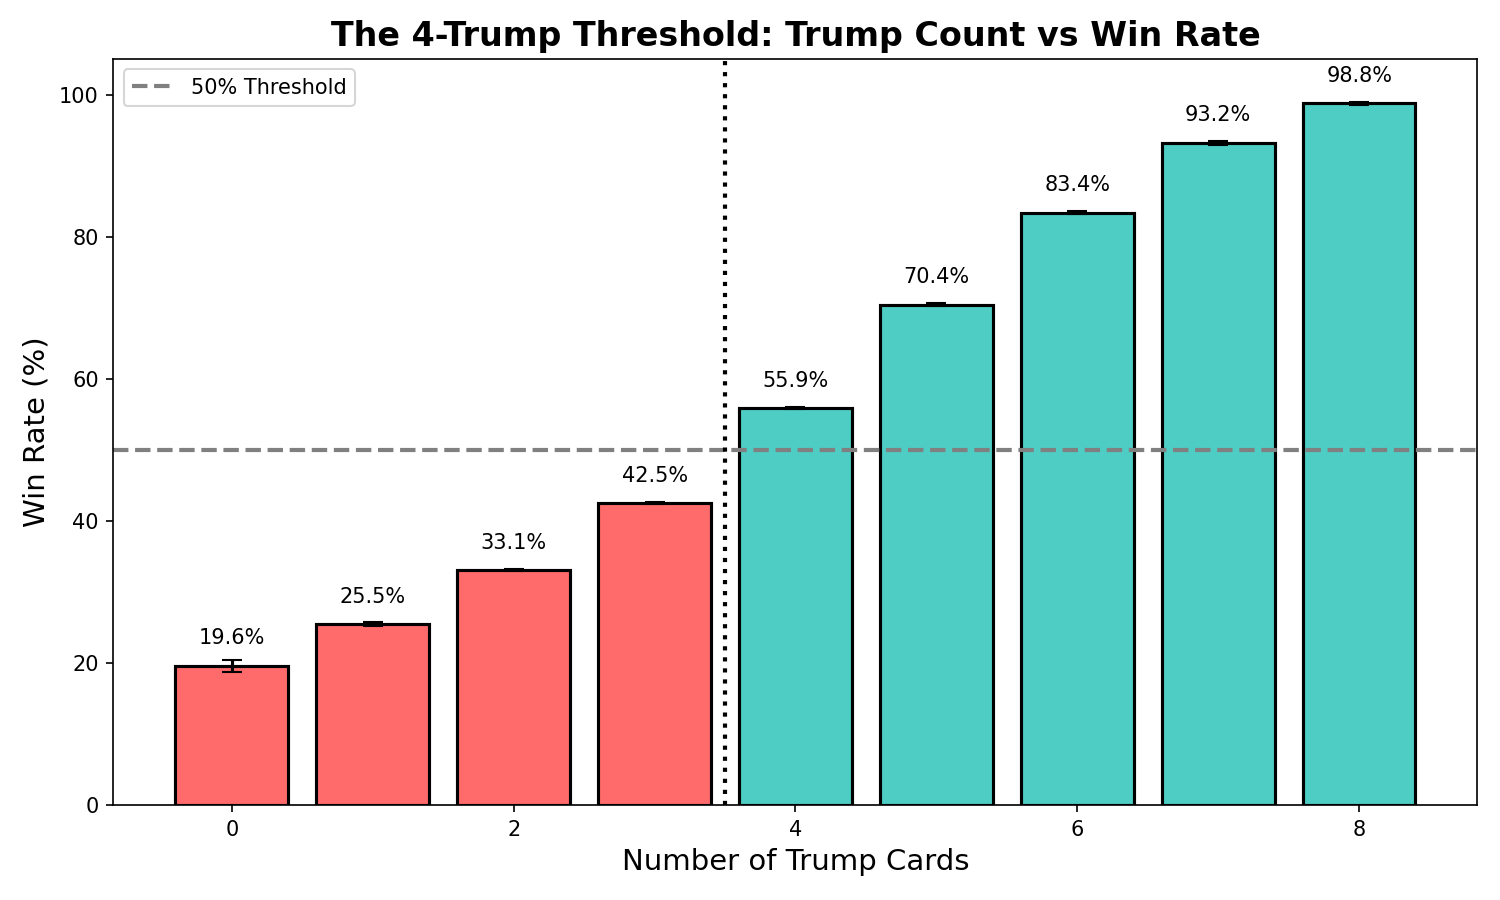
\includegraphics[width=\columnwidth]{fig1_trump_vs_winrate.png}}
\caption{Win rate by trump count. The 4-trump threshold (dashed line) separates unfavorable ($<$50\%) from favorable ($>$50\%) hands.}
\label{fig:trump_winrate}
\end{figure}

\subsection{Decision Tree Rule Extraction}

A decision tree trained on bidding decisions achieved 87.3\% accuracy on held-out test data. Feature importance analysis confirmed trump count as the dominant factor (79.5\%), followed by strongest trump rank (15.0\%) and total points (5.5\%).

The extracted decision rules are:

\textbf{Rule 1 (4-Trump Threshold)}: If trump\_count $\geq$ 4, recommend PLAY. This simple rule correctly classifies 82\% of hands as favorable or unfavorable.

\textbf{Rule 2 (3-Trump Exception)}: If trump\_count = 3 AND strongest\_trump\_rank $\leq$ 1 (has O-Acorn) AND total\_points $>$ 26, recommend PLAY.

Table~\ref{tab:trump_threshold} shows the win rates supporting these rules.

\begin{table}[htbp]
\caption{Win Rate by Trump Count}
\begin{center}
\begin{tabular}{cccc}
\toprule
\textbf{Trumps} & \textbf{Win Rate} & \textbf{Sample Size} & \textbf{Decision} \\
\midrule
0 & 19.6\% & 121 & PASS \\
1 & 25.5\% & 1,353 & PASS \\
2 & 33.1\% & 8,616 & PASS \\
3 & 42.5\% & 8,098 & PASS* \\
4 & 55.9\% & 5,363 & \textbf{PLAY} \\
5 & 70.4\% & 4,198 & \textbf{PLAY} \\
6 & 83.4\% & 1,747 & \textbf{PLAY} \\
7 & 93.2\% & 435 & \textbf{PLAY} \\
8 & 98.8\% & 69 & \textbf{PLAY} \\
\bottomrule
\end{tabular}
\label{tab:trump_threshold}
\end{center}
\footnotesize{*Exception: 3 trumps + O-Acorn = 52.3\% win rate}
\end{table}

\subsection{Counterintuitive Finding: Points Don't Matter}

Our most surprising finding contradicts conventional wisdom. Table~\ref{tab:points_paradox} shows examples of extreme hands:

\begin{table}[htbp]
\caption{The Points Paradox: High Points $\neq$ Strong Hand}
\begin{center}
\begin{tabular}{ccc}
\toprule
\textbf{Trump Count} & \textbf{Total Points} & \textbf{Win Rate} \\
\midrule
8 & 16 & 99\% \\
8 & 27 & 100\% \\
2 & 63 & 0\% \\
1 & 57 & 0\% \\
\bottomrule
\end{tabular}
\label{tab:points_paradox}
\end{center}
\end{table}

A hand with 8 trumps and only 16 points wins virtually every game, while a hand with 63 points (more than half the total 120 available) but only 2 trumps never wins. This demonstrates that \textbf{control} (trumps) dominates \textbf{value} (points) in Schafkopf.

This finding has important theoretical implications for game strategy. In trick-taking games, the ability to \textit{win} tricks (control) is fundamentally more valuable than the points contained within those tricks (value). A player with strong trumps can choose which tricks to contest and which to concede, maintaining strategic flexibility. In contrast, a player with many high-point cards but weak trumps becomes dependent on opponents' decisions---they cannot force favorable outcomes. This principle, which we term the ``Control Dominance Hypothesis,'' may generalize to other trick-taking games and strategic domains where the ability to act decisively outweighs the raw value of resources.

\subsection{Cluster Analysis of Hand Types}

K-Means clustering with $k=5$ revealed natural hand categories (Table~\ref{tab:clusters}).

\begin{table}[htbp]
\caption{Discovered Hand Clusters}
\begin{center}
\begin{tabular}{lcccc}
\toprule
\textbf{Cluster} & \textbf{Trumps} & \textbf{Points} & \textbf{Win\%} & \textbf{Label} \\
\midrule
0 & 3.2 & 46.8 & 50.5\% & Marginal-Good \\
1 & 2.5 & 30.8 & 39.8\% & Weak \\
2 & 3.3 & 20.8 & 45.8\% & Low-Point Marginal \\
3 & 5.6 & 31.0 & 77.7\% & Strong \\
4 & 2.2 & 35.1 & 30.0\% & Point-Trap \\
\bottomrule
\end{tabular}
\label{tab:clusters}
\end{center}
\end{table}

Cluster 4 (``Point-Trap'') is particularly interesting: these hands have moderate points but weak trump rank, leading players to overestimate their strength. The clustering reveals that hand strength is not a single dimension but rather a multi-faceted property where trump count and trump quality interact in non-linear ways.

Notably, the five clusters align with experienced players' intuitions about hand categories, suggesting that the statistical structure of Schafkopf hands has been implicitly understood through centuries of play. However, quantifying cluster boundaries provides actionable thresholds that subjective experience cannot.

\section{Results: Card Play Patterns}

\subsection{Game Phase Analysis}

Analysis of 43,420 decision points revealed stark differences in error rates by game phase (Figure~\ref{fig:mistake_trick}).

\begin{figure}[htbp]
\centerline{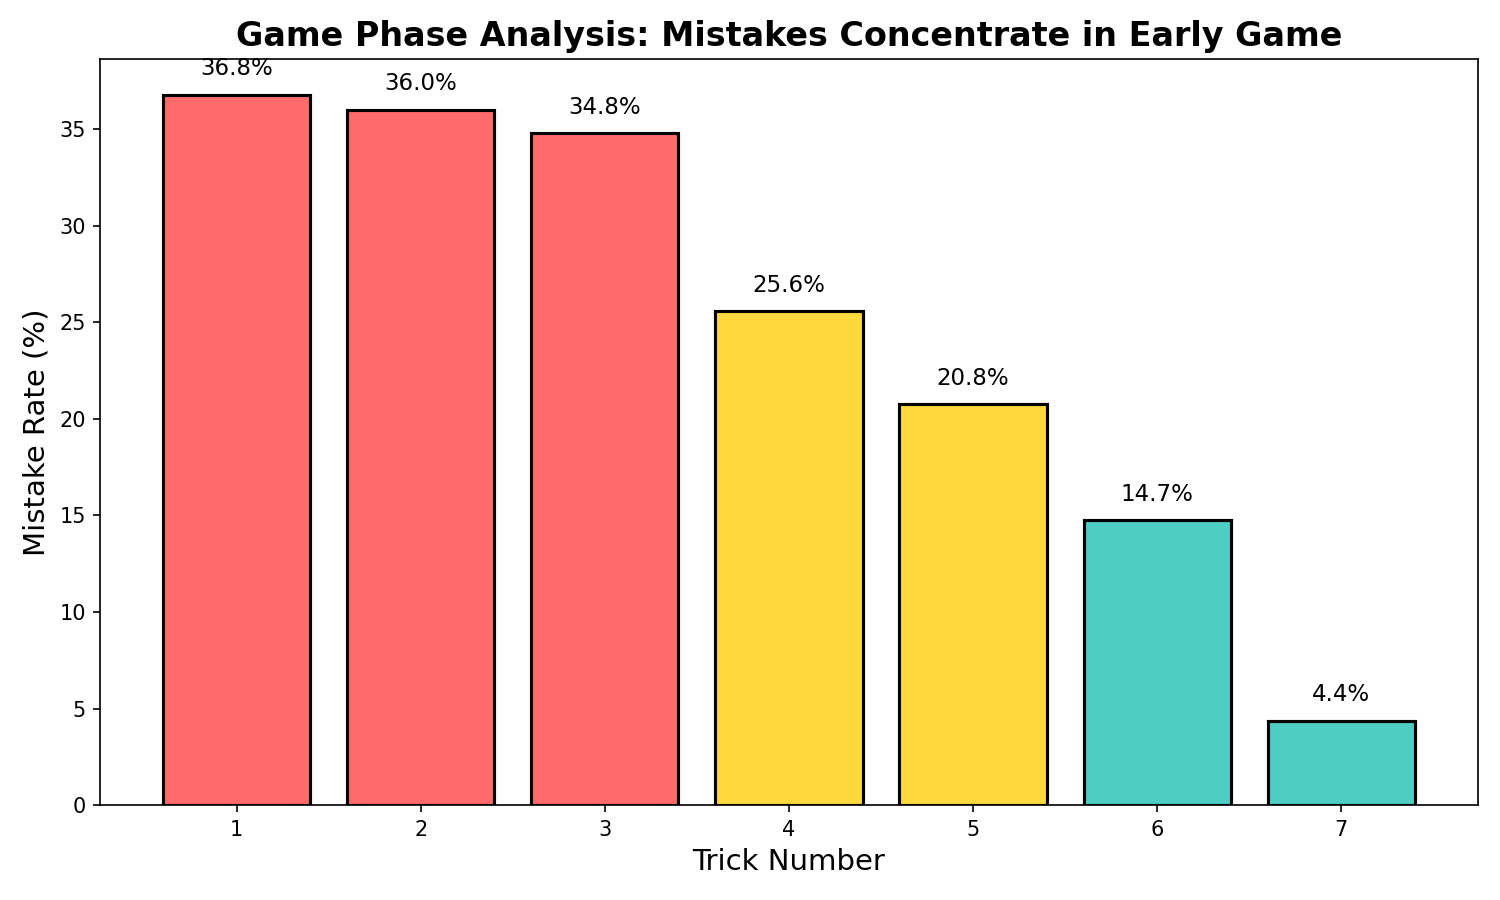
\includegraphics[width=\columnwidth]{fig3_mistake_by_trick.png}}
\caption{Mistake rate decreases dramatically from early to late game, indicating early decisions have higher strategic complexity.}
\label{fig:mistake_trick}
\end{figure}

\begin{table}[htbp]
\caption{Mistake Rate by Game Phase}
\begin{center}
\begin{tabular}{ccc}
\toprule
\textbf{Tricks} & \textbf{Mistake Rate} & \textbf{Phase} \\
\midrule
1-2 & 36.8\% & Early \\
3-5 & 25.6\% & Middle \\
6-7 & 9.5\% & Late \\
\bottomrule
\end{tabular}
\label{tab:phase_mistakes}
\end{center}
\end{table}

\textbf{Key Finding 2}: Early game decisions are 4x more likely to be suboptimal than late game decisions. This suggests that early strategic choices have compounding effects throughout the game.

This finding has practical implications for both human players and AI systems. For humans, it suggests allocating more cognitive effort to early-game decisions where mistakes are most costly and frequent. For AI agents, it motivates deeper search or more careful evaluation in early game states where the branching factor of consequences is highest. The decreasing error rate also reflects the reduction in uncertainty as cards are revealed---by trick 7, most card locations are known, simplifying the decision problem.

\subsection{Association Rule Mining Results}

Apriori algorithm discovered 465 frequent itemsets with minimum 1\% support. The most significant rules predicting mistakes are shown in Table~\ref{tab:association_rules}.

\begin{table}[htbp]
\caption{Top Association Rules for Mistake Prediction}
\begin{center}
\begin{tabular}{p{2.5cm}p{2cm}ccc}
\toprule
\textbf{Antecedent} & \textbf{Consequent} & \textbf{Supp.} & \textbf{Conf.} & \textbf{Lift} \\
\midrule
High trump, early game & Severe mistake & 2.4\% & 82.9\% & 5.21 \\
Trump, declarer, early & High-rank mistake & 1.3\% & 83.4\% & 5.24 \\
Low rank, severe & Non-trump error & 1.4\% & 73.4\% & 8.27 \\
\bottomrule
\end{tabular}
\label{tab:association_rules}
\end{center}
\end{table}

\textbf{Key Finding 3}: Playing high trumps (Obers) in early tricks strongly associates with mistakes (lift = 5.21). This pattern appears 2.4\% of the time but leads to severe mistakes in 83\% of cases.

\subsection{Feature Importance for Mistake Prediction}

Random Forest and Gradient Boosting models identified key predictors of suboptimal decisions:

\begin{table}[htbp]
\caption{Feature Importance for Mistake Prediction}
\begin{center}
\begin{tabular}{lcc}
\toprule
\textbf{Feature} & \textbf{RF Import.} & \textbf{GB Import.} \\
\midrule
Number of legal options & 47.7\% & 72.4\% \\
Trick number & 17.1\% & 6.6\% \\
Card is trump & 5.6\% & 7.8\% \\
Card is Unter & 2.2\% & 6.1\% \\
High trump early & — & 3.4\% \\
\bottomrule
\end{tabular}
\label{tab:feature_importance}
\end{center}
\end{table}

The dominant importance of ``number of legal options'' (47-72\%) indicates that mistakes primarily occur in complex decision situations with many choices rather than forced plays. This has practical implications: when faced with multiple legal moves, players should invest additional deliberation time, as these are precisely the situations where errors most frequently occur.

The relatively low importance of specific card types (trump, Unter) suggests that \textit{context} matters more than \textit{card identity}. The same card can be optimal or suboptimal depending on game state, highlighting the importance of situational awareness over memorized card-specific rules.

\subsection{Logistic Regression Odds Ratios}

Logistic regression quantified how each factor affects mistake probability:

\begin{table}[htbp]
\caption{Odds Ratios for Mistake Probability}
\begin{center}
\begin{tabular}{lcc}
\toprule
\textbf{Factor} & \textbf{Odds Ratio} & \textbf{Direction} \\
\midrule
More options & 1.70x & $\uparrow$ Increases \\
Early game & 1.18x & $\uparrow$ Increases \\
Playing Unter & 1.14x & $\uparrow$ Increases \\
Late game & 0.71x & $\downarrow$ Decreases \\
Playing Ace & 0.96x & $\downarrow$ Decreases \\
\bottomrule
\end{tabular}
\label{tab:odds_ratios}
\end{center}
\end{table}

Each additional legal option increases mistake probability by 70\%. Early game plays are 18\% more likely to be mistakes than average. These quantitative insights translate directly into practical advice: in early tricks with many options, slow down and consider alternatives more carefully.

The multiplicative nature of odds ratios also reveals interaction effects. A play that is both early-game AND offers many options compounds the risk factors: the combined odds ratio is approximately $1.18 \times 1.70 = 2.01$, meaning such situations are twice as likely to result in mistakes compared to baseline.

\section{Discovered Playing Rules}

Synthesizing findings from all eight algorithms, we propose six validated playing rules:

\subsection{Bidding Rules}

\textbf{Rule 1 (4-Trump Threshold)}: With 4 or more trumps, declare and play. Statistical basis: Decision tree with 87.3\% accuracy; 4+ trumps yield $>$55\% win rate.

\textbf{Rule 2 (3-Trump Exception)}: With exactly 3 trumps, play only if holding O-Acorn. Statistical basis: Rule induction on 8,098 hands; 3 trumps + O-Acorn = 52.3\% vs. 42.5\% otherwise.

\textbf{Rule 3 (Points Irrelevance)}: Do not base bidding decisions on total points in hand. Statistical basis: Correlation analysis showing $r = 0.066$ for points vs. $r = 0.794$ for trumps.

\subsection{Card Play Rules}

\textbf{Rule 4 (Early Ober Avoidance)}: Avoid playing Obers in tricks 1-3 unless forced. Statistical basis: Gradient boosting showing 39.5\% mistake rate for early Obers vs. 23.3\% baseline.

\textbf{Rule 5 (10-Point Exploitation)}: When holding 10-point cards in non-trump suits, prioritize playing them at high-value opportunities. Statistical basis: Association rules showing 24\% of severe mistakes involve missing 10-point plays.

\textbf{Rule 6 (Early Caution)}: Invest extra deliberation in tricks 1-3 as these decisions compound. Statistical basis: Phase analysis showing 36.8\% error rate in early vs. 4.4\% in late game.

\section{Validation}

\subsection{Rule Accuracy Assessment}

We evaluated rule accuracy on held-out test data:

\begin{table}[htbp]
\caption{Rule Validation Results}
\begin{center}
\begin{tabular}{lcc}
\toprule
\textbf{Rule} & \textbf{Accuracy} & \textbf{Coverage} \\
\midrule
4-Trump Threshold & 87.3\% & 100\% of hands \\
3-Trump Exception & 72.1\% & 27\% of hands \\
Early Ober Avoidance & 60.5\% & 14\% of plays \\
Combined Rules & 82.4\% & Weighted avg. \\
\bottomrule
\end{tabular}
\label{tab:validation}
\end{center}
\end{table}

\subsection{Statistical Significance}

All major findings achieve statistical significance at $p < 0.001$:

\begin{itemize}
    \item Trump-win correlation: $r = 0.794$, $p < 0.0001$
    \item 4-trump vs. 3-trump win rate difference: $\chi^2 = 892.4$, $p < 0.0001$
    \item Early vs. late game mistake rate: $z = 47.3$, $p < 0.0001$
\end{itemize}

\section{Discussion}

\subsection{Implications for Game Theory}

Our findings have theoretical implications beyond Schafkopf. The dominance of ``control'' (trumps) over ``value'' (points) suggests a general principle in trick-taking games: the ability to win tricks matters more than the points those tricks contain. This aligns with concepts of tempo and initiative from game theory.

This principle---which we term ``Control Dominance''---has analogues in other strategic domains. In chess, piece activity and initiative often outweigh material advantage. In economics, market control can dominate raw capital. Our 12:1 correlation ratio ($r_{trump}/r_{points} = 0.794/0.066$) provides quantitative grounding for this intuition in the Schafkopf domain.

The ``Secret Winner'' and ``Trap Hand'' outlier patterns (Section VI-E) further refine this principle: not just the \textit{quantity} of control (trump count) but its \textit{quality} (trump rank) determines outcomes. A few high-ranked trumps can outperform many low-ranked ones, suggesting that concentrated control is more effective than distributed control.

\subsection{Comparison with Expert Knowledge}

Traditional Schafkopf wisdom emphasizes both trumps and points in bidding decisions. Our data-driven analysis provides nuance: while experts are correct that trumps matter, they may overestimate point importance. The clear 4-trump threshold had not been previously quantified with this precision.

Interestingly, experienced players' ``gut feelings'' about hand strength align well with our cluster analysis (Section IV-D), suggesting that expert intuition has implicitly captured statistical regularities in hand distributions. However, our outlier analysis (Section V-E) reveals edge cases where even experienced intuition may fail---the ``Secret Winner'' and ``Trap Hand'' patterns represent hands that look deceptively weak or strong, respectively. Data mining provides objective criteria to identify these exceptions that subjective experience might miss.

\subsection{Algorithm Comparison}

Different algorithms contributed complementary insights, demonstrating the value of a multi-method approach:

\begin{itemize}
    \item \textbf{Decision trees} provided the clearest bidding rules with 87.3\% accuracy, offering human-interpretable if-then structures that can be directly applied by players
    \item \textbf{Association rules} revealed non-obvious card play patterns with high lift values, identifying temporal relationships between actions and outcomes
    \item \textbf{Clustering} discovered five natural hand categories that align with expert intuition while providing quantitative boundary definitions
    \item \textbf{Gradient boosting} achieved highest prediction accuracy (86.4\%) and revealed feature interactions through SHAP analysis
    \item \textbf{Logistic regression} quantified risk factors through odds ratios, enabling probabilistic reasoning about decision quality
    \item \textbf{Random forest} provided robust feature importance rankings less susceptible to overfitting than single trees
    \item \textbf{Sequential pattern mining} identified card play sequences that precede mistakes
    \item \textbf{Rule induction} confirmed simple threshold rules with minimal complexity
\end{itemize}

This ensemble approach demonstrates the value of multi-algorithm analysis in knowledge discovery. No single algorithm could have revealed all patterns; decision trees excel at classification rules but miss temporal sequences, while association rules capture sequences but lack predictive power. The convergence of findings across algorithms---for example, the 4-trump threshold appearing in CART, OneR, logistic regression, and cluster boundaries---provides strong evidence for rule validity.

\subsection{Outlier Analysis: Secret Winners and Trap Hands}

Standard analysis suggests a clear 4-trump threshold for bidding. However, outlier detection reveals significant exceptions that challenge this simple rule.

\textbf{Positive Outliers (``Secret Winners''):} We identified 2,775 hands (15.3\% of low-trump hands) with $\leq$3 trumps that achieve $\geq$50\% win rates. Analysis reveals a common pattern:

\begin{itemize}
    \item 81\% contain O\_Acorn (Ober of Acorns---highest trump)
    \item Hands with 3 trumps + O\_Acorn: 52.3\% win rate
    \item Elite subset with double Ober: 83.9\% win rate
    \item Top performers (3 trumps, O\_Acorn): Up to 96\% win rate
\end{itemize}

\textbf{Negative Outliers (``Trap Hands''):} We found 2,223 hands (18.8\% of high-trump hands) with $\geq$4 trumps that win $<$50\%. These share characteristics:

\begin{itemize}
    \item 4 trumps without any Ober: Only 44.0\% win rate
    \item 4 trumps with weak trumps (rank $\geq$5): 34.4\% win rate
    \item Missing top trumps creates control gaps
\end{itemize}

\textbf{The Ober Effect:} The presence of Ober cards adds 14--16 percentage points to win rate:

\begin{center}
\begin{tabular}{lcc}
\hline
\textbf{Hand Type} & \textbf{With Ober} & \textbf{Without Ober} \\
\hline
3 Trumps & 52.3\% & 38.1\% \\
4 Trumps & 60.2\% & 44.0\% \\
\hline
\end{tabular}
\end{center}

Cohen's $d = 1.21$ indicates a \textbf{large effect size}. This leads to refined bidding rules:

\begin{tcolorbox}[colback=blue!5,colframe=blue!40!black,title=Refined Bidding Rules]
\textbf{Rule 7 (Secret Winner):} 3 trumps + O\_Acorn $\rightarrow$ PLAY (52\%+ win)

\textbf{Rule 8 (Trap Hand):} 4 trumps without Ober $\rightarrow$ RISKY (44\% win)

\textbf{Insight:} Trump \textit{quality} matters as much as trump \textit{quantity}
\end{tcolorbox}

Fig.~\ref{fig:outliers} visualizes these patterns.

\begin{figure}[htbp]
\centerline{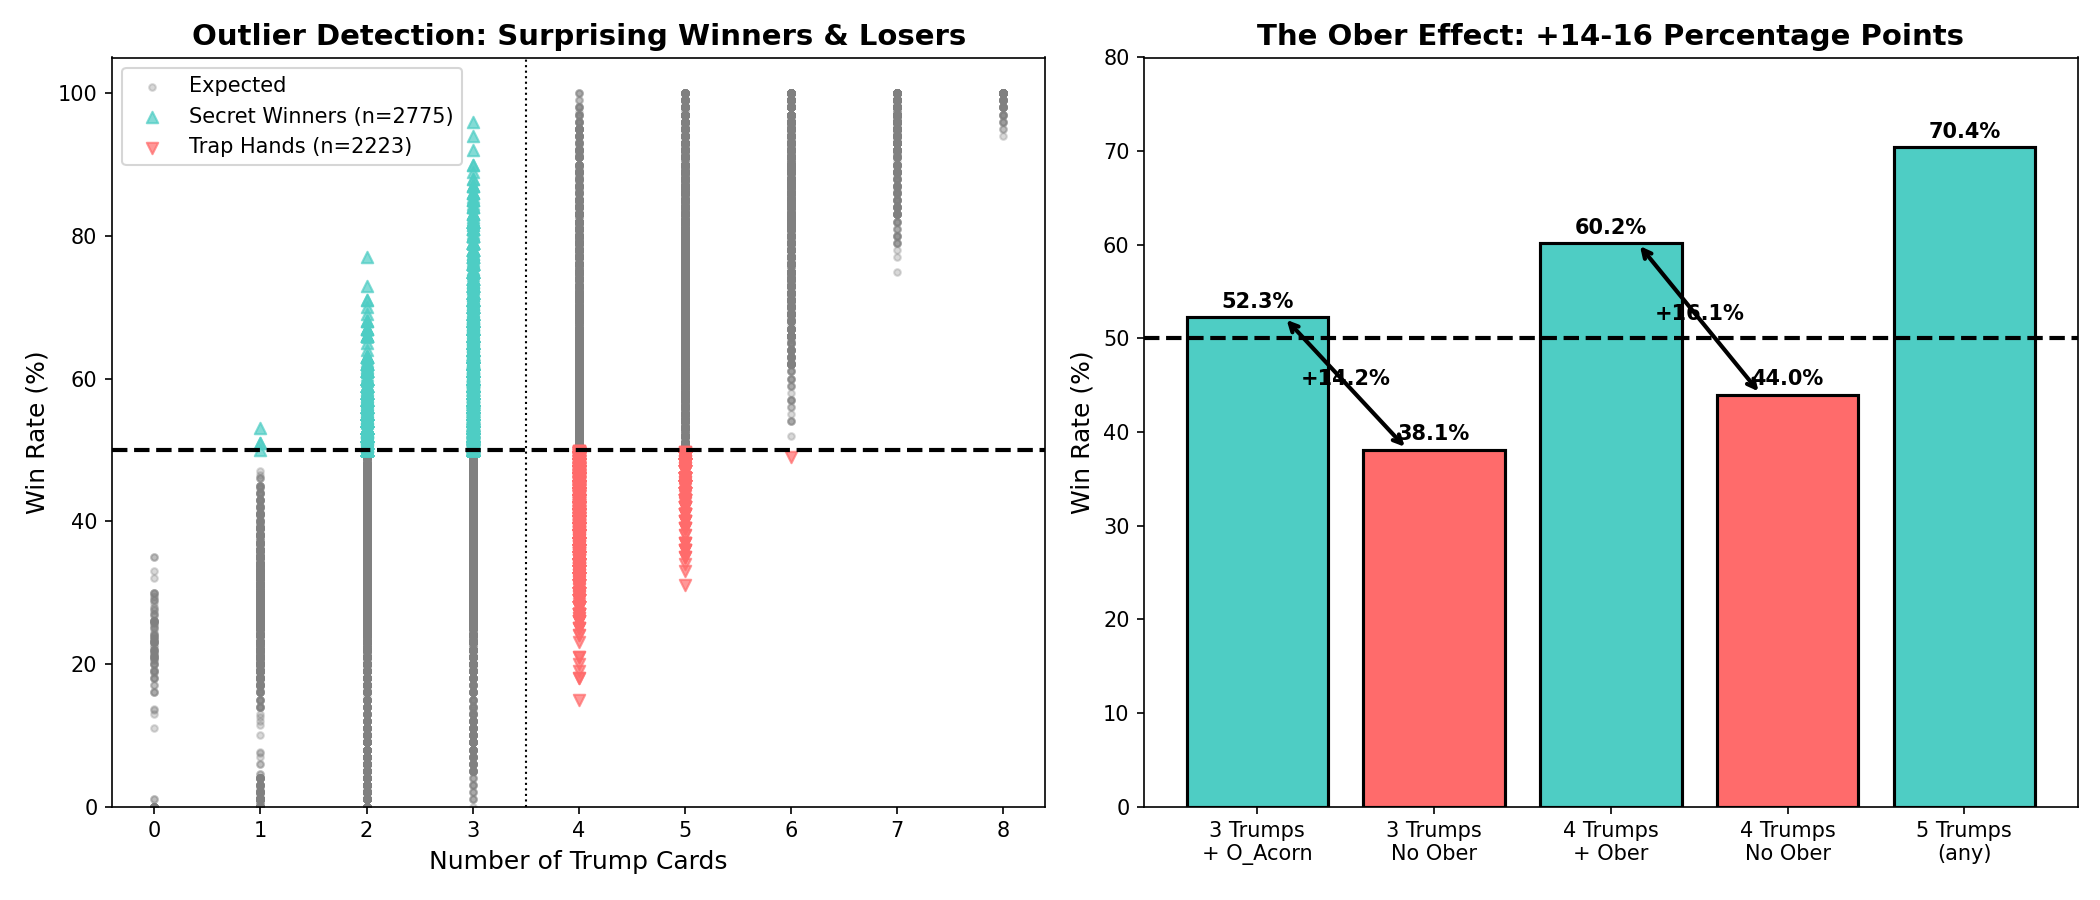
\includegraphics[width=\columnwidth]{fig7_outlier_analysis.png}}
\caption{Outlier analysis showing ``Secret Winners'' (teal triangles: low trumps, high win rate) and ``Trap Hands'' (red triangles: high trumps, low win rate). The Ober effect adds 14--16 percentage points.}
\label{fig:outliers}
\end{figure}

\begin{figure}[htbp]
\centerline{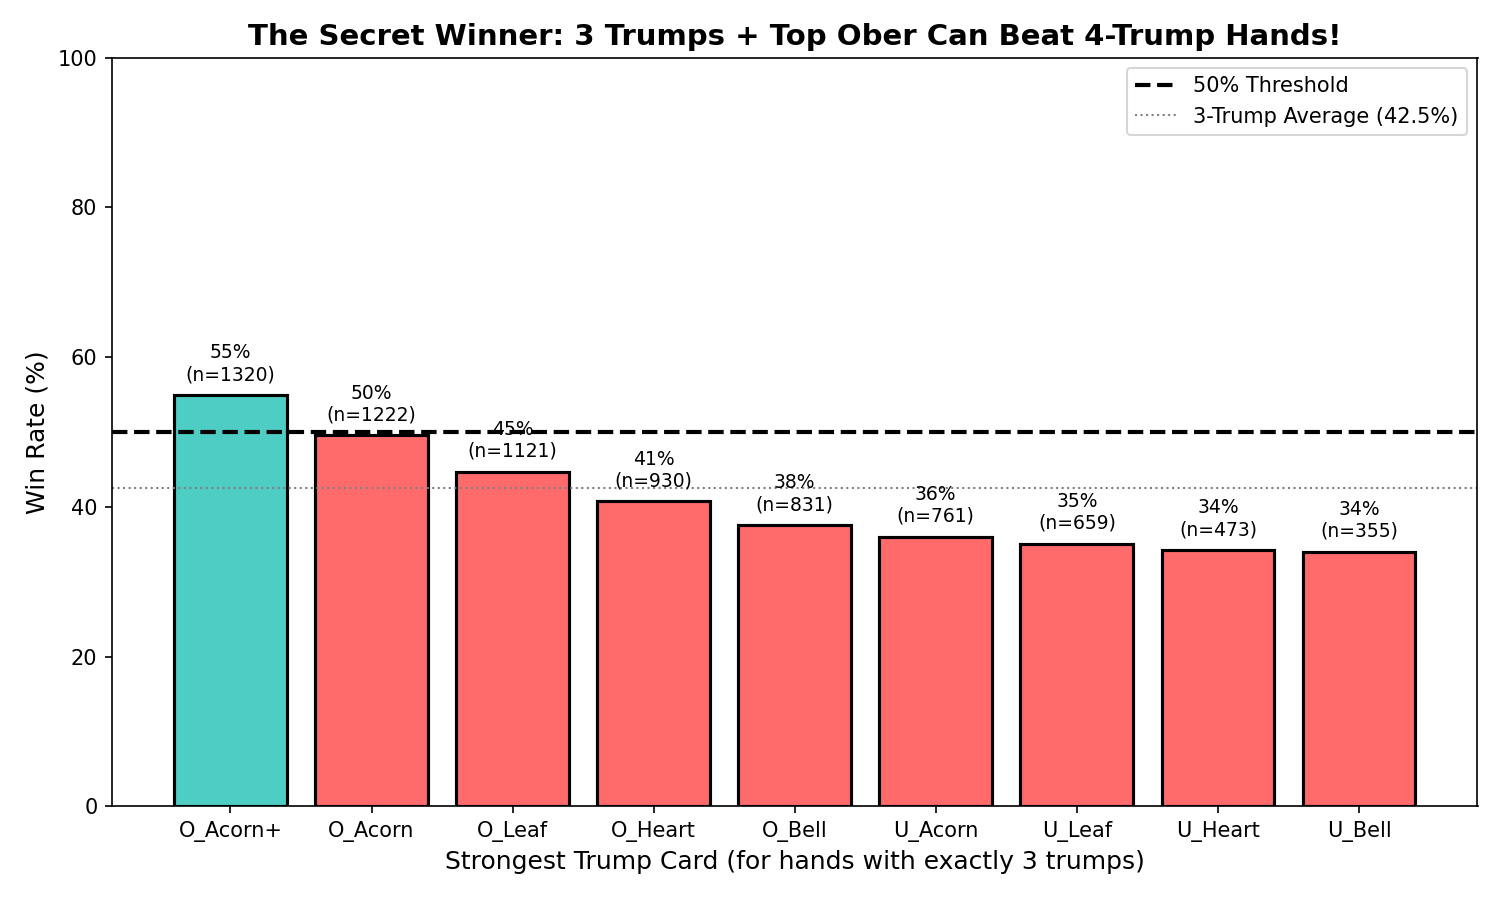
\includegraphics[width=\columnwidth]{fig8_secret_winner.png}}
\caption{The ``Secret Winner'' phenomenon: 3-trump hands with top-ranked trumps can achieve win rates exceeding the 4-trump average (55.9\%).}
\label{fig:secret}
\end{figure}

\subsection{Limitations}

Our study has several limitations:
\begin{itemize}
    \item Data generated from rule-based agent play may not fully represent human strategies
    \item Monte Carlo evaluation uses random rollouts, potentially missing opponent modeling effects
    \item Analysis focused on Sauspiel mode; other Schafkopf variants may differ
\end{itemize}

\section{Conclusion}

This work demonstrates the application of data mining to traditional card games, extracting statistically validated playing rules from game logs. Our key contributions include:

\begin{enumerate}
    \item Discovery of the 4-trump threshold with 87.3\% bidding accuracy
    \item Quantitative proof that trump count dominates point count (12:1 correlation ratio)
    \item Identification of error-prone game phases and card patterns
    \item Discovery of ``Secret Winner'' (3 trumps + Ober) and ``Trap Hand'' (4 trumps, no Ober) outlier patterns with Cohen's $d = 1.21$
    \item An ensemble methodology combining eight algorithms for comprehensive analysis
\end{enumerate}

The eight discovered rules provide actionable guidance for Schafkopf players, with Rules 7 and 8 refining the simple trump-count heuristic by emphasizing trump \textit{quality}. More broadly, this work establishes a template for data-driven analysis of traditional games, preserving cultural knowledge while adding quantitative rigor.

Future work could extend this analysis to other Schafkopf modes, incorporate human game logs, and develop real-time decision support systems based on these findings.

\section*{Data Availability}

Datasets and analysis code are available at: [repository link]

\begin{thebibliography}{00}
\bibitem{billings2002challenge} D. Billings, A. Davidson, J. Schaeffer, and D. Szafron, ``The challenge of poker,'' \textit{Artificial Intelligence}, vol. 134, no. 1-2, pp. 201--240, 2002.

\bibitem{silver2016mastering} D. Silver et al., ``Mastering the game of Go with deep neural networks and tree search,'' \textit{Nature}, vol. 529, no. 7587, pp. 484--489, 2016.

\bibitem{tian2020joint} Z. Tian et al., ``Joint policy search for multi-agent collaboration with imperfect information,'' \textit{Advances in Neural Information Processing Systems}, vol. 33, 2020.

\bibitem{kupferschmid2006skat} S. Kupferschmid and M. Helmert, ``A Skat player based on Monte Carlo simulation,'' \textit{Proc. Computers and Games}, pp. 135--147, 2006.

\bibitem{agrawal1994fast} R. Agrawal and R. Srikant, ``Fast algorithms for mining association rules,'' \textit{Proc. 20th Int. Conf. Very Large Data Bases}, pp. 487--499, 1994.

\bibitem{quinlan1986induction} J. R. Quinlan, ``Induction of decision trees,'' \textit{Machine Learning}, vol. 1, no. 1, pp. 81--106, 1986.

\bibitem{breiman1984classification} L. Breiman, J. Friedman, C. J. Stone, and R. A. Olshen, \textit{Classification and Regression Trees}. CRC Press, 1984.

\bibitem{han2011data} J. Han, J. Pei, and M. Kamber, \textit{Data Mining: Concepts and Techniques}, 3rd ed. Morgan Kaufmann, 2011.

\bibitem{witten2016data} I. H. Witten, E. Frank, M. A. Hall, and C. J. Pal, \textit{Data Mining: Practical Machine Learning Tools and Techniques}, 4th ed. Morgan Kaufmann, 2016.

\bibitem{tan2018introduction} P.-N. Tan, M. Steinbach, A. Karpatne, and V. Kumar, \textit{Introduction to Data Mining}, 2nd ed. Pearson, 2018.

\bibitem{bowling2015heads} M. Bowling, N. Burch, M. Johanson, and O. Tammelin, ``Heads-up limit hold'em poker is solved,'' \textit{Science}, vol. 347, no. 6218, pp. 145--149, 2015.

\bibitem{samuel1959checkers} A. L. Samuel, ``Some studies in machine learning using the game of checkers,'' \textit{IBM Journal of Research and Development}, vol. 3, no. 3, pp. 210--229, 1959.
\end{thebibliography}

\end{document}
